\documentclass[8pt]{extarticle}
\usepackage[utf8]{inputenc}
\usepackage{blindtext}
\usepackage{multicol}
\usepackage[landscape=true, a4paper, margin=1cm]{geometry}
\usepackage{enumitem}
\usepackage{graphicx}

\pagestyle{empty}
\graphicspath{ {./images} }

\usepackage[dvipsnames]{xcolor}
\setitemize{itemsep=-0.1cm}

\title{Zusammenfassung AnTeDe}
\author{Florian Bär}
\date{June 2022}

\begin{document}

% \maketitle

% \section{Introduction}
\begin{multicols*}{3}
[
%\section{AnTeDe Zusammenfassung}
]

\textbf{1} Frame the problem and look at the big picture.
\textbf{2} Get the data.
\textbf{3} Explore the data to gain insights.
\textbf{4} Prepare the data to better expose the underlying data patterns to ML algorithms.
\textbf{5} Explore many different models and short-list the best ones.
\textbf{6} Fine-tune your models and combine them into a great solution.
\textbf{7} Present your solution.
\textbf{8} Launch, monitor, and maintain your system.
\newline \textbf{Text analysis draws on knowledge from several fields}
\begin{itemize}
    \item algorithmics, statistics, machine learning
    \item computational linguistics, corpus linguistics
    \item human computer interaction, interface design
\end{itemize}
\textbf{Text analysis} is artificial intelligence (AI) applied to \textbf{human language}
\newline \textbf{Utterance} can be understood by decoding the propositional content (it's logical form)
\newline Text is build of letters $\rightarrow$ syllables $\rightarrow$ morphemes (a meaningful part of a word like in, come, -ing) $\rightarrow$ words $\rightarrow$ phrases (a group of words together e.g. after dinner) $\rightarrow$ clauses (a group of words containing a subject and a verb) $\rightarrow$ sentences (simple sentence, compound sentence, complex sentence) $\rightarrow$ texts $\rightarrow$ corpora
\newline \textbf{Components of text analysis}
\newline \textbf{Lexical analysis} - clean textual data and extract
\newline \textbf{Syntactic analysis} - interpret relationships \& grammatical structures
\newline \textbf{Semantic analysis} - find meaning and interpret individual sentences
\newline \textbf{Discourse analysis} - find meaning across sentences
A \textbf{Token} is an occurrence of a word, a \textbf{type} is the base form of a word (lemma)
\newline $\frac{\textrm{Type}}{\textrm{Token}}$ -Ratio expresses the lexical diversity
\newline \textbf{Text-Classification} can be done by \textbf{Handcoded Rules} or \textbf{Supervised ML}
\newline A set of document $D$, classes $c$, a training set of $M$ labeled documents $(d_1, c_1),...$ where the output is a mapping $D \rightarrow C$
\newline \textbf{Cond. probabilty} $P(A) P(B|A) = P(A \cap B) = P(B \cap A) = P(B) P(A | B)$
\newline \textbf{bayesian theorem} $ P(A|B) = \frac{P(B|A)P(A)}{P(B)}$
\newline \textbf{Naïve Bayes Classifier}: $P(c|d) = \frac{P(d|c)P(c)}{P(d)}$
\newline $c_{NB} = \textrm{argmax} P(c) \prod_{k=1}^{N} P(x_k | c) $ 
\newline \textbf{Maximum A Posteriori}: $\textrm{argmax} P(d|c) P(c)$
\newline \textbf{Bernoulli}: is word present or not
\newline \textbf{Multinomial}: how many occurrences of word i in d
\newline \textbf{feature independence}: $P(x_1, x_2, ..., x_N | c) = P(x_1 | c) P(x_2 | c) ... P(x_N | c)$
\newline $P(c)$ can be calculated based on the maximum likelihood
\newline $P(x_i | c)$ can be estimated as $\frac{\textrm{\# occ. of token i in c}}{\textrm{total \# of tokens in c}} = \frac{\textrm{\# occ. of token i in c + 1}}{\textrm{total \# of tokens in c + V}}$ where \textbf{V is the count of all tokens in the vocabulary} which is \textbf{Laplace smoothing}
\newline \textbf{Prior} = prob. of class in Training $\rightarrow$ \textbf{posterior} = occ. of w in class
\newline Prior = $\frac{1}{3}$, Post = $\frac{\textrm{bear in Bern} + 1}{\textrm{\#w in class Bern + \#w in corpus}}$
\newline to prevent \textbf{underflow} use the log probabilities bc. of small numbers 
\newline $ c_{NB} = \textrm{argmax}_{c \in C} log(P(c) + \sum_{k = 1}^N log(P(x_k | c) $
\newline \textbf{Accuracy} $\frac{TP + TN}{TP + TN+ FN + FP}$
\newline \textbf{Precision for class} $\frac{TP}{TP + FP}$ - fraction of test documents classified as c that have been correctly classified
\newline \textbf{Recall for class} $\frac{TP}{TP + FN}$ - fraction of test documents labeled as c that have been correctly classified
\newline \textbf{F1 Score for class} $\frac{2 P_c R_c}{P_c + R_c}$ - harmonic mean of P and R

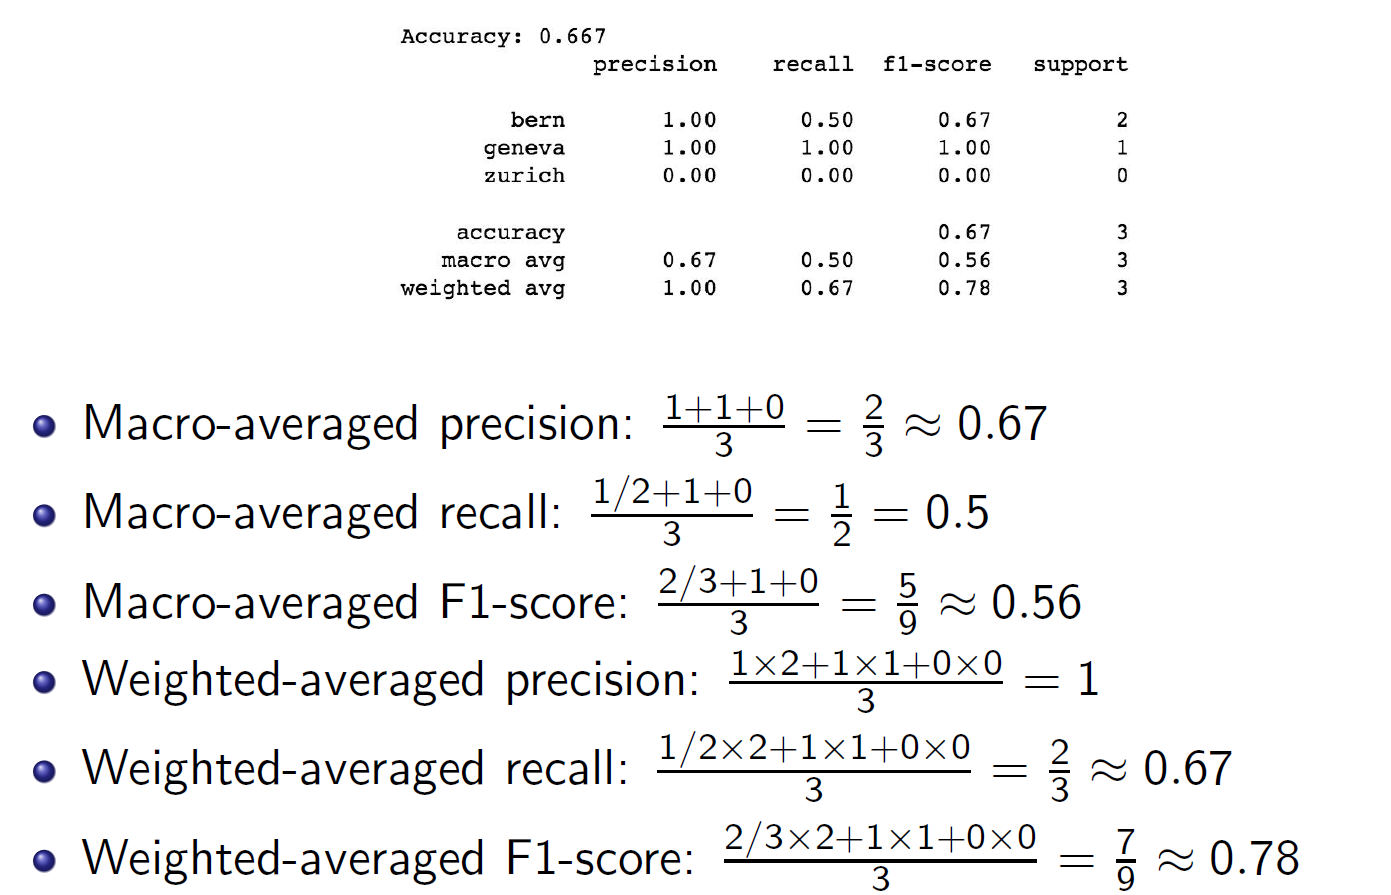
\includegraphics[width=0.75\columnwidth]{macro_weighted.png}
\textbf{If the predicted are the cols and true are rows}
\newline \textbf{Accuracy}: trace (sum of elements along the main diagonal) over grand sum (sum of all elements)
\newline \textbf{Precision}: given a column (i.e., a predicted label), element on main diagonal over sum of matrix column
\newline \textbf{Recall}: given a row (i.e., a test label), element on main diagonal over sum of matrix row

\textbf{Sentiment analysis} is hard! It consists of \textbf{opinion holder}, \textbf{target entity} (Movie), \textbf{aspect} (What feature), \textbf{type} (pos, neg) and the \textbf{time} when it was expressed
\newline Check for emojis, yaaaaay (length normalization), multiword expressions (buckle up babay), \textbf{negations} (What you said is not NOT\_true. - till end of the sentence)
\newline Check for \textbf{modal adverbs} (quite, totally), \textbf{expectations} (i guess you think...), \textbf{non-literal language} (like 50 hours long)
\newline $PMI(w_1, w_2) = log_2 (\frac{P(w_1, w_2)}{P(w_1) P(w_2)}) = log_2(\frac{P(w_2 | w_1)}{P(w_2)})$ 
\newline $PMI = \frac{\textrm{Comb. Res * all Res (normalize)}}{\textrm{Res W1 * Res W2}}$ $\rightarrow$ high PMI = together
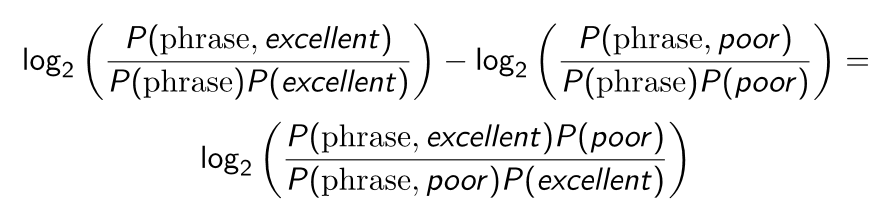
\includegraphics[width=0.75\columnwidth]{pmi}
\newline \textbf{Information retrieval} with a boolean model can not be ranked
\newline Vector-Space Model - word (row) -document (col) - Matrix or Term-Term Matrix (occ. in Window)
\newline \textbf{TF} Occurrences of W in D - use \textbf{dampening}
\newline $TF, ln(1 + TF), \frac{TF(k+1)}{k+TF}$ as TF (k = pos. Const.)
\newline \textbf{IDF} = $\frac{1}{\textrm{number of d containig type = DF}}$
\newline $IDF = ln(\frac{\# D}{DF}), ln(\frac{\# D}{1 + DF}), 1 + ln(\frac{\# D}{DF})$ (\# D is \# of D in Corpus)
\newline \textbf{Doc length normaliz} $ DLN = (1 - b) * \# D / \textrm{avg doc len} $ b $ \in $  [0,1]
\newline $ \textrm{similarity}=\cos(\theta )={\mathbf {A} \cdot \mathbf {B}  \over \|\mathbf {A} \|\|\mathbf {B} \|}={\frac {\sum \limits _{i=1}^{n}{A_{i}B_{i}}}{{\sqrt {\sum \limits _{i=1}^{n}{A_{i}^{2}}}}{\sqrt {\sum \limits _{i=1}^{n}{B_{i}^{2}}}}}}$
\newline $ {\text{jaccard}}= \frac{\sum \limits _{i=1}^{n} min(v_1, w_i)}{\sum \limits _{i=1}^{n} max(v_1, w_i)}$
\newline $ {\text{dice}}= \frac{2 \times \sum \limits _{i=1}^{n} min(v_1, w_i)}{\sum \limits _{i=1}^{n} (v_1 + w_i)}$
\newline $ {\text{Jensen-Shannon}}= D(\overrightarrow{v} | \frac{\overrightarrow{v} + \overrightarrow{w}}{2}) + D(\overrightarrow{w} | \frac{\overrightarrow{v} + \overrightarrow{w}}{2})$
\newline if $ |\overrightarrow{v}| = 1$ \textbf{cosine sim} is v(q) * v(d)
\newline \textbf{Okapi BM25} {\displaystyle {\text{s}}(D,Q)=\sum _{i=1}^{n}{\text{IDF}}(q_{i})\cdot {\frac {f(q_{i},D)\cdot (k_{1}+1)}{f(q_{i},D)+k_{1}\cdot \left(1-b+b\cdot {\frac {|D|}{\text{avgdl}}}\right)}}}
\newline \textbf{or} s(q,d) $= \sum \frac{\textrm{tf-idf(t,d)}}{|d|}$
\newline 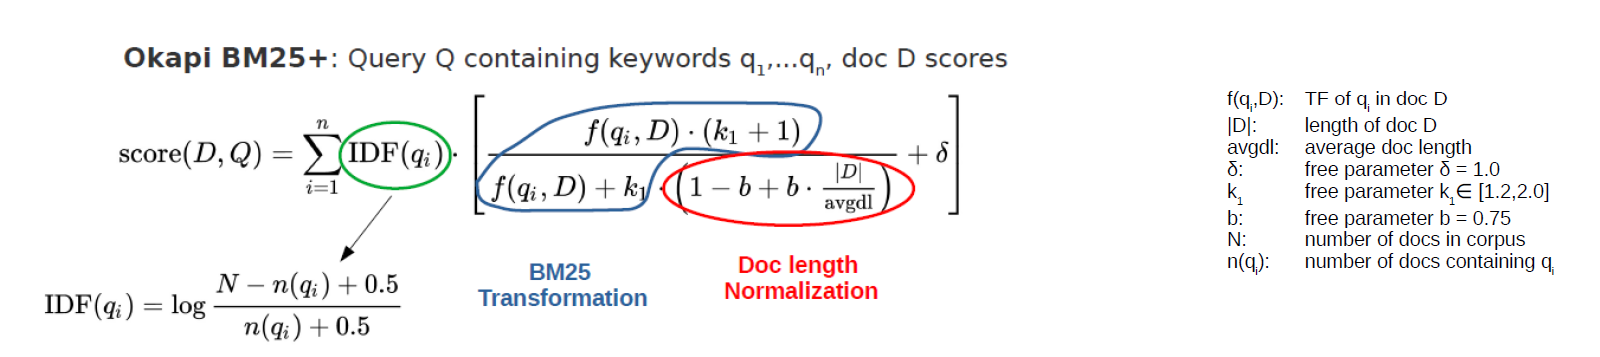
\includegraphics[width=0.9\columnwidth]{okapi}
\newline \textbf{Machine learning models}
\newline\textbf{Pointwise approaches} : learn scores
\newline \textbf{Pairwise approaches} : also learn scores, but with different loss functions
\newline \textbf{Listwise approaches} : consider the ranked list in its entirety
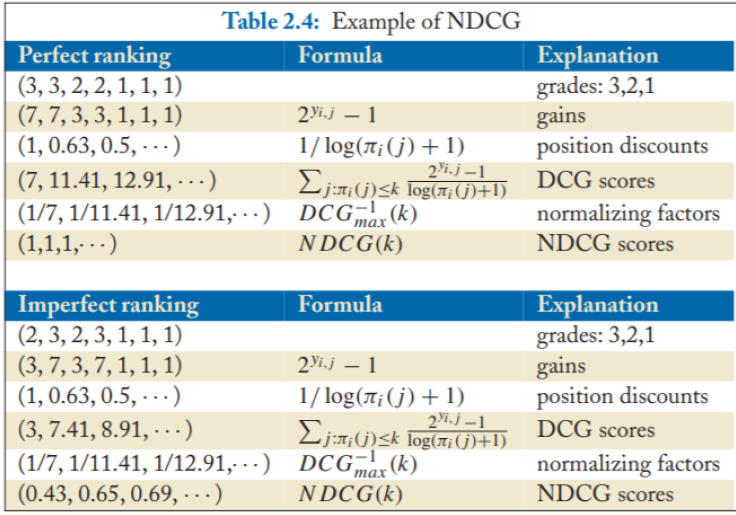
\includegraphics[width=0.6\columnwidth]{ndcg}
\newline Missing: word order, semantic similarity, polysemy (apple, bush)
\newline \textbf{Latent Semantic Analysis} (uses SVD)
\newline SVD $ \rightarrow M = U \times \sum \times V^t$
\newline M =  term document matrix
\newline U = $5 \times 5$, Rotation Matrix
\newline $\sum = m \times n $, Coord by Coord Scaling (Singular Values)
\newline V^t = $ n \times n $, Rotation 
\newline Shrink $\sum$ Matrix to save storage (sparse to dense) and find synonyms
\newline \textbf{word2vec} learns embeddings for hidden layer ($200-500 size_h$)
\newline use \textbf{CBOW} (w given n) or \textbf{Skip-Gram} (n given w)
\newline $ v_w_i  = W^T \cdot x_w_i = h_w_i  $ and $W'^{T} \cdot h_w_i = u_w_i$
\newline $ p(o|c) = \frac{e^{v_c^T \cdot u_o}}{\sum_{w \in V} e^{v_c^T \cdot u_w}}$
\newline better convergance, negative samples! else \textbf{degenerate} solution
\newline For Skip-Gram 1. define context window, 2. stopwords downsampling, 3. take $W$ and $W'$ - 5-20 for small dataset, 2-5 else
\newline 3 possibilties: 1. discard $w'$, 2. sum the embeddings, 3. concatenate
\newline \textbf{analogy analysis} $=$ kitty - cute = cat
\newline WS $\sim$ 5 same topic, WS $\sim$ 2 same category
\newpage
\textbf{POS} has 9 main categories, the open and closed ones: \textbf{open} (nouns, verbs, adjectives, adverbs, interjections), \textbf{close} (pronouns, prepositions, conjunctions, determiners)
\newline used for Txt2Speech and opposite, word sense disambiguation, syntactical parsing, information extraction, question answering, MT
\newline \textbf{CC} - coordinating conjuction, \textbf{DT} - Determiner, \textbf{JJ} - Adjective, \textbf{MD} - Modal, \textbf{NN} - Noun (singular), \textbf{NNS} - Noun (plural), \textbf{NNP} - proper noun, \textbf{NNPS} - proper noun (plural), \textbf{PRP} - personal Pronoun, \textbf{VB} - verb, \textbf{VBD} - verb past tense, \textbf{VBG} - verb gerund, \textbf{VBP} - verb non 3rd singular present, \textbf{VNZ} - verb 3rd present singular
\newline Hidden Markov Model (hidden states not known) 
\newline just multiply all the possibilities to get the probability of the sequence
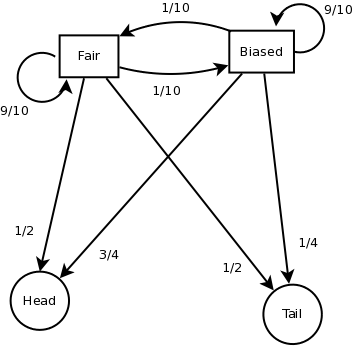
\includegraphics[width=0.4\columnwidth]{fairbet}
\newline A = Transition Matrix (hidden states/tags) B = emission matrix (observations, word given the state)
\newline $\pi_{fair}$ as starting point * Emmision * $\textrm{State}_{\textrm{Transition}}$ etc. How likely is our seq. of h. states done our sequence? Try all, take best prob.
\newline HMM (Markovity $\rightarrow$ only depend on tag before, Output independence $\rightarrow$ output only depend on state!)
\newline $a_{0,1} = P_{VBP|PRP} \approx \frac{\textrm{# of PRP VBP}}{\textrm{# of PRP}}$
\newline $b_{1,2} = P_{VBP|PRP} \approx \frac{\textrm{# of word tagged as VBP}}{\textrm{# of VBP}}$
\newline \textbf{Viterbi algorithm} (Trellis graph, row = tag, column = word)
\newline First row (in A) is the $\pi$ probability
\newline Check in the B Matrix, which Tag the next word can be!
\newline \textbf{Language Models} speech to text, spell correction, word prediction
\newline \textbf{Perplexity } lower is better 
\newline Perplexity is probability of test set, normalized by the \# of words - avg. branching factor
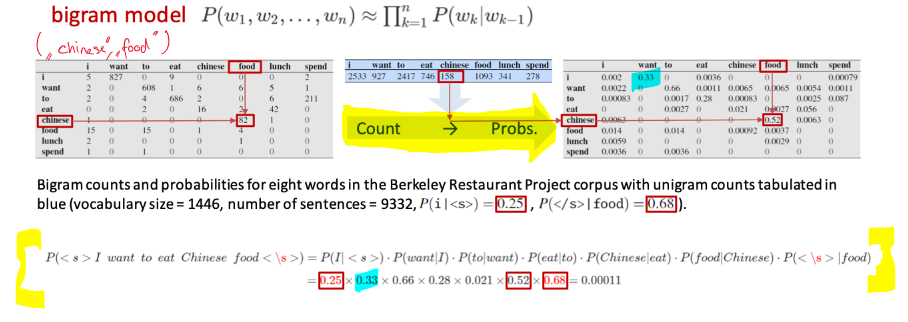
\includegraphics[width=\columnwidth]{bigram_model}
Problem with unknown words $\rightarrow$ probabitlity is 0
\newline use Laplace smoothing for unknown words

\newline Text generation $ \rightarrow $ sample randomly given the distribution
\newline \textbf{Feedforward LM} use markov assumption! but slower
\newline \textbf{RNN} uses hidden states  (BPTT)
\newline Gradients can vanish (GRU, LSTM) or explode (clipping)!! 
\newline syntactical parsing (understanding text) T $\rightarrow$ terminals (words), N $\rightarrow$ nonterminals (labels as NounPhrase, VerbPhrase)
\newline \textbf{NounPhrase} (the smart dog), \textbf{Verbphrase} (went home), \textbf{prepositional phrase} (at home, after dinner), \textbf{adjective / adverb phrase} (very politically correct), \textbf{clause} (I'm going home) , \textbf{Sentence} (build of multiple clauses) simple, compound, complex
\newline \textbf{constituent} move words around - check what stays together!
\newline \textbf{S} simple clause, \textbf{SBAR} (i think (that) i'm stupid), \textbf{SBARQ} (direction questions starting with a WH-word), \textbf{SINV} (never has so much been owed), \textbf{SQ} (yes no questions)
\newline \textbf{dependency parsing} main idea is the root
\newline \textbf{Shift} (move a word from top of buffer to top of stack)
\newline \textbf{Left arc} (nb of the head of stack is dependent to head of stack, add link to dep. graph with label, remove nb from stack)
\newline \textbf{Right arc} (head of stack is dependent on nb, add link to dep graph with label, remove head of stack)
\newline [stack][buffer] - init stack with [root] and buffer with words
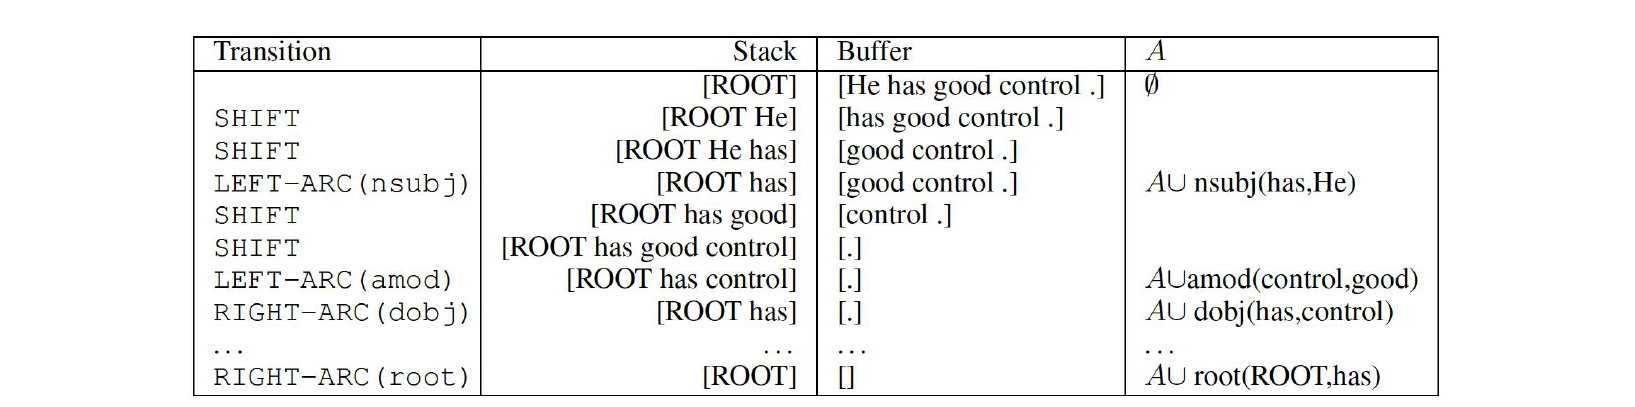
\includegraphics[width=\columnwidth]{arc}
\newline noun modifier, nominal subject, direct object
\newline use svn, nn, to determine operation!
\newline \textbf{UAS} unlabeled attachment score (dependency correct)
\newline \textbf{LAS} labeled attachment score (and labels rights) smaller!!
\newline \textbf{character based LM} uses $<$UNK$>$ for unknown words
\newline use Bi-LSTM (this text and text this)
\newline \textbf{fasttext uses Chracter and word based LM}
\newline create \textbf{subwords} by number of occurrences. add the bigrams (first the ones with the highest counts)
\newline \textbf{BPE} Byte Pair Encoding is smaller than language model (used by main LM, MachineTranslation)
\newline \textbf{Attention} Multiply hidden states with decoder hidden state, use a \textit{softmax}, concat attention with hidden state $\frac{e^{z}}{\sum e^z_j}$
\newline there is a multiplicate and a additive attention
\newline \textbf{decode} with greedy search, exhaustive search or \textbf{beam search}
\newline With the \textbf{beam search}, only expand the K words with highest score!
\newline \textbf{BLEU} matches only ngrams, not order of grams
\newline The Bilingual Evaluation Understudy compares the machine written translation to one or several human written translations and computes a similarity score, Measures the ratio of matched n-grams (overlap) to the total number of n-grams in the translated text (range [0..1] but often scaled to [0..100]), Typically 1,2,3 and 4-gram precision which are equally weighted, Penalty for translations that are too short using a brevity penalty (BP) factor
\newline \colorbox{BurntOrange}{EXAMPLE HERE for calculation}
\newline \textbf{Transformer} stacks (MH Attention, add-norm, feed forward, add-norm) with 6 blocks (add-norm = resid) not shared weights!!
\newline use q, k and v (score = q $\times$ k), then softmax and then $\times$ value!
\newline positional encoding is done with \textbf{sin} and \textbf{cos}
\newline \textbf{Information extraction} NER, coreference resolution, entity linking, relation extraction, event extraction, template filling
\newline \textbf{NER} - I-Type, O, B-Type, E-Type, S-Type (Singleton) and can then used for \textbf{IO} (n + 1 tags) and \textbf{IOB} (2n +1) $\rightarrow$ n = all types of tags
\newline use \textbf{HMM} (generative) or \textbf{MEMM} (max entropy) (discriminative)
\newline \textbf{Discriminative}, log-linear model for NER that uses softmax, + Easier to condition on new features, - Disadvantage: Suffers from label bias problem = Viterbi algo disregards local
\newline Viterbi uses states with less transitions!
\newline use conditional random fields \textbf{CRF}
\newline \textbf{CRF} overcomes the label bias problem by using unnormalized scores locally (potentials),
instead of probabilities, and a global normalizer. Can be used to top of a neural network → thus still relevant
\newline do feature extraction (prefixes/suffixes) of words $\rightarrow$ short shapes (Americans = Xx, of = x, AMR = X (TLA), . = .)
\newline \textbf{Contextual word embeddings} (ELMo - use all available hidden layers) uses transfer learning
\newline Natural Language Inference (Recognizing Textual Entailment) ("madonna is alone" = contradiction) (contradiction, neutral, entailment) and Semantic role labeling (extracts key relationships)
\newline \textbf{GPT} uses only decoder, \textbf{BERT} uses only encoder
\newline distill models with teacher (big model) to train student (small model (factor 50))
\newline Coreference resultion: I visit your grave. X is dead for 4 years. x=you?
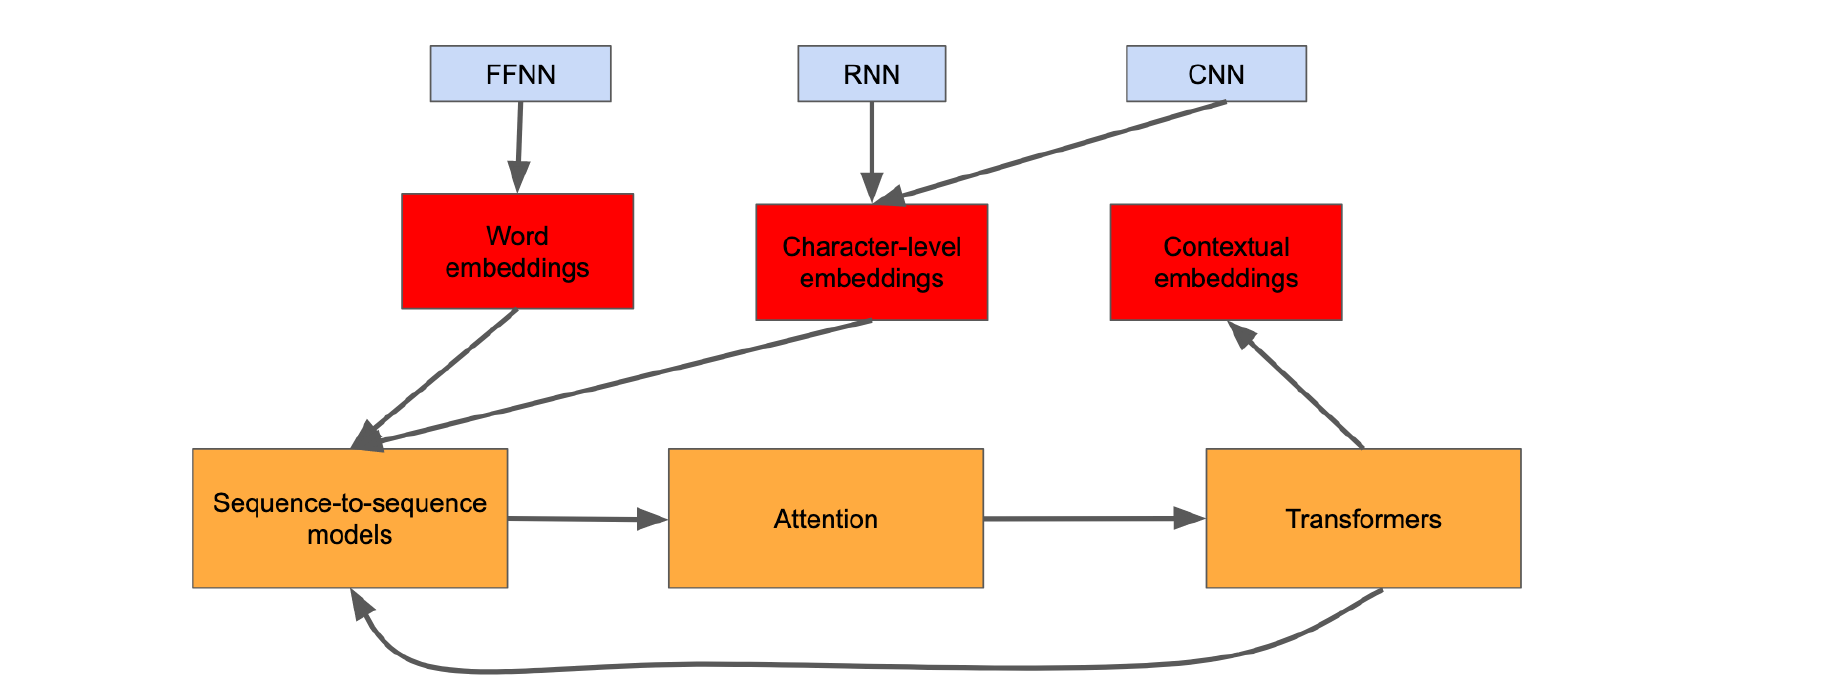
\includegraphics[width=\columnwidth]{models}
\textbf{Task oriented dialogue agents} (closed domain) and \textbf{chatbots}
\newline A dialog is a sequence of turns: \textbf{constatives} (answering, claim, deny), \textbf{directives} (advise, ask, forbid, invite), \textbf{commissives} (promise, plan, betting, opposing) and \textbf{acknowledgements} (apologize, greet, thank)
\newline Response by retrieval (find similar responses) or response by generation (encoder, decoder)
\newline 2010 chatbots lack of personality, lack of long-term memory!
\newline chirpy SOTA chatbot AWS, TransferTransfo HuggingFace (autoreggresive  = one token at the time)
\newline 2 Head Model does 2 tasks (e.g. LM prediction and next sentence prediction - make sentence and recheck)
\newline Persona-Chat Dataset (given person and then chat together)
\newline zero-shot (only persona), Few-Shot (persona, couple examples), one-shot (persona and 1 example)
\newline \textbf{ELIZA} Uses “Rogerian psychology”, where the chatbot knows almost nothing about the world and asks everything -  I was on a board ride - Tell me about boats
\newline \textbf{ULMFiT} (Universal language modelling for text classification)
\newline Use large corpus to pre-train a large LM, then fine-tune LM to target domain,- freeze the weights of large LM and add a task-specific classification head for specific task, \textbf{With this approach}, much less data is required to reach a certain performance
\newline \textbf{ELMo}, Two BiLSTM layers with 4096 units and residual connections between the two
\newline \textbf{Beam Search} uses $ log(P_{LM}(got | <start> I) + \textrm{value before}$
\newline \textbf{Probability of Sentence} $P(w_1 | w_2, w_3) = \frac{P(w_1, w_2, w_3)}{P(w_2, w_3)} $
\end{multicols*}

\end{document}
